\documentclass{beamer}

%% Use package -----------------------------------------------------------------

\usepackage[T1]{fontenc}
\usepackage[utf8]{inputenc}
\usepackage{lmodern}
\usepackage{graphicx}
\usepackage[absolute,overlay]{textpos}
\usepackage{multicol}
\usepackage{listings}
\usepackage{svg}

%% Beamer customization---------------------------------------------------------

\usepackage{xcolor}
\usetheme{Warsaw}

%% Themes
% Outer themes
\useoutertheme{shadow}
% Rounded boxes and shadows
\useinnertheme[shadow=true]{rounded}
% Solid \item symbols
\useinnertheme{circles}

%% Custom colors
\definecolor{rltgreen}{rgb}{0,0.5,0}
\definecolor{pasteur}{RGB}{0,90,154}
\setbeamerfont{block title}{size={}}
\setbeamercolor{structure}{fg=pasteur}
\setbeamercolor{item}{fg=pasteur}

%Color of title
\setbeamertemplate{frametitle}
{
    \nointerlineskip
    \begin{beamercolorbox}[sep=0.3cm,ht=1.8em,wd=\paperwidth]{frametitle}
        \vbox{}\vskip-2ex%
        \strut\insertframetitle\strut
        \vskip-0.8ex%
    \end{beamercolorbox}
}
% Hide navigation symbols
\setbeamertemplate{navigation symbols}{}

%% Title block
\setbeamercolor*{title}{use=structure,fg=white,bg=pasteur}

%% Bottom infolines
\setbeamertemplate{footline}
{
  \leavevmode%
  \hbox{%
  \begin{beamercolorbox}[wd=.3\paperwidth,ht=2.25ex,dp=1ex,center]{author in head/foot}%
    \usebeamerfont{author in head/foot}\insertshortauthor
  \end{beamercolorbox}%
  \begin{beamercolorbox}[wd=.7\paperwidth,ht=2.25ex,dp=1ex,center]{title in head/foot}%
    \usebeamerfont{title in head/foot}\insertshorttitle\hspace*{3em}
    \insertframenumber{} / \inserttotalframenumber\hspace*{1ex}
  \end{beamercolorbox}}%
  \vskip0pt%
}
\makeatletter

%% Top infolines
\setbeamertemplate{headline}{%
\leavevmode%
  \hbox{%
    \begin{beamercolorbox}[wd=\paperwidth,ht=2.5ex,dp=1.125ex]{palette quaternary}%
    \insertsectionnavigationhorizontal{\paperwidth}{}{\hskip0pt plus1filll}
    \end{beamercolorbox}%
  }
}
\setlength{\leftmargini}{10pt}
%% Define Snakemake ------------------------------------------------------------

\definecolor{eclipseBlue}{RGB}{42,0.0,255}
\definecolor{eclipseGreen}{RGB}{63,127,95}
\definecolor{eclipsePurple}{RGB}{127,0,85}

\lstset{language=Python}
\lstset{
    basicstyle=\tiny\ttfamily,
    morekeywords={rule, output, shell, params, run, configfile, temp},
    showstringspaces=false,
    commentstyle=\color{eclipseGreen}, % style of comments
    keywordstyle=\color{eclipsePurple}, % style of keywords
    stringstyle=\color{eclipseBlue}, % style of strings
}


%% Set up title ----------------------------------------------------------------

\title{Sequana: a set of NGS pipelines}
\subtitle{overview and status (Feb-Aug 2016)}
\author[T.Cokelaer \& D.Desvillechabrol]{Thomas Cokelaer and Dimitri Desvillechabrol}
\institute{Institut Pasteur}
\date{Sept 13th 2016}

\begin{document}

%% Title slide -----------------------------------------------------------------

\begin{frame}[plain]
    \titlepage
    \begin{textblock*}{5cm}(4.5cm,0.3cm)
        
\includegraphics[scale=0.09]{Institut_Pasteur.png}
    \end{textblock*}
\end{frame}

%% Slides ----------------------------------------------------------------------



\begin{frame}
 \frametitle{Sequana: a set of NGS pipelines}
 \framesubtitle{teszt}
 \begin{columns}
 \begin{column}{0.48\textwidth}
\tiny 
\begin{block}{Overview}
\begin{itemize}
 \item  In the context of the Biomics platform, we are developing NGS pipelines 
 to analyse DNA sequencing data (Illumina). Pipelines are 
available within the \textbf{Sequana} project.\\
\item  We aim at providing HTML reports and clean processed data that 
are reproduceable but also a common  library  to 
foster co-development within IP.\\
\item Currently, we have  pipelines to assess the quality of the sequences, 
detect variants, denovo assembly, taxonomic content, systematic 
study of the assembly coverage. \\
\item A Continuous Integration guarantees a high quality software (reproducibility, tests, doc)
\end{itemize}
\end{block}

 \begin{exampleblock}{\tiny Timeline and usage}
    \tiny
    \begin{itemize}
      \item Sequana Project started in March 2016 and is entering production mode for the PF1 platform.
      \item Currently, Sequana is used to analyse paired or single-end Illumina seq. data (HiSeq, MiSeq)
      \item Future pipelines will include long reads analysis.
      \item Sequana can be used on the BIC or Tars IP cluster. A release is planed by the end of 2016
      \end{itemize}
  \end{exampleblock}


\end{column}

\begin{column}{0.5\textwidth}
 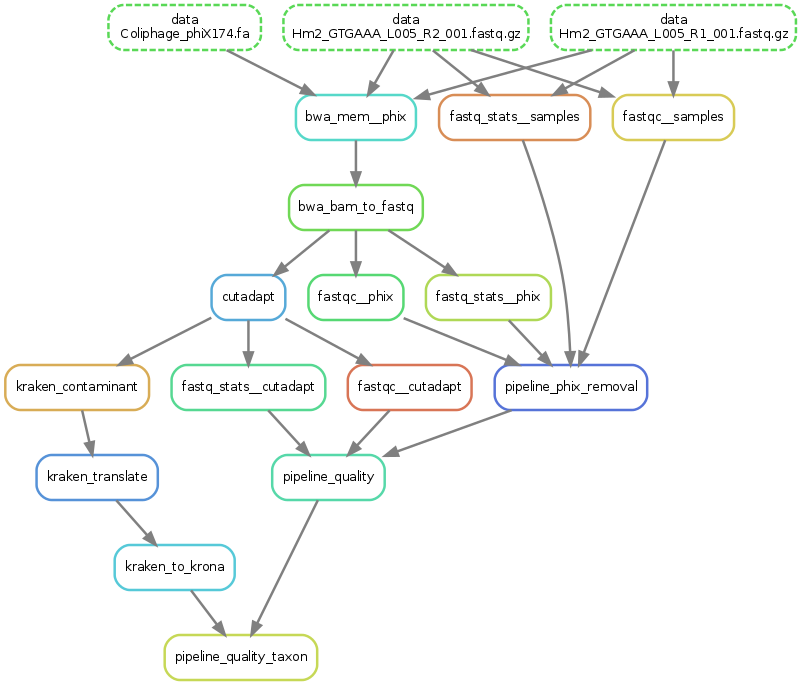
\includegraphics[scale=0.14, height=6em]{pipeline}
  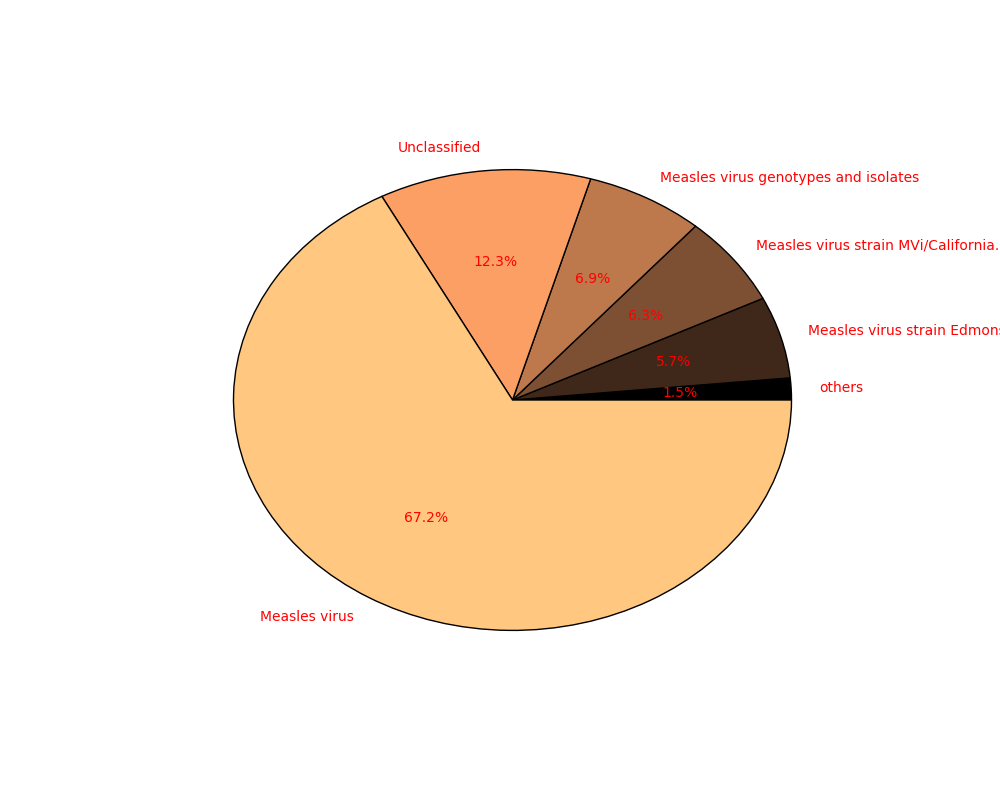
\includegraphics[scale=0.14]{kraken}\\
  
\includegraphics[scale=0.15]{coverage}
  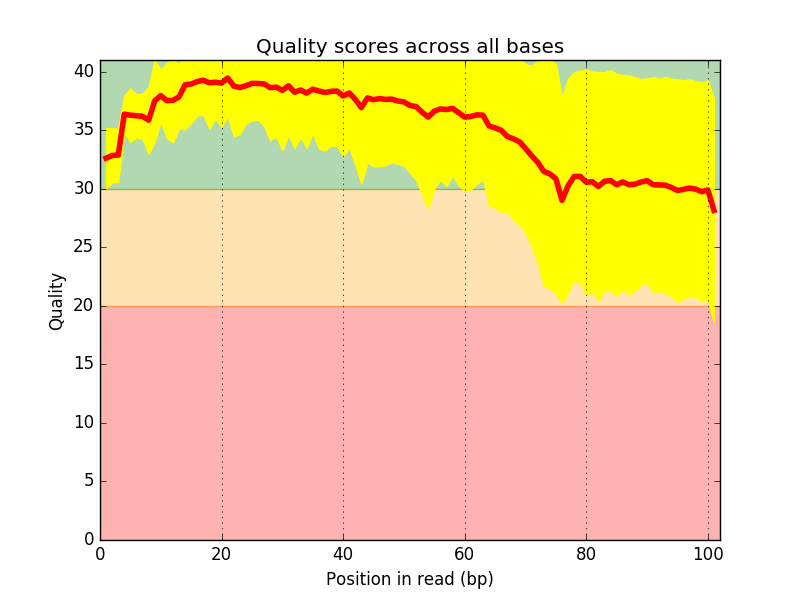
\includegraphics[scale=0.15]{fastqc}

  
  \begin{block}{\tiny Links and contributions}
    \tiny
    \begin{itemize}
      \item For developers, please join the github  : https://github.com/sequana/sequana    
      \item For users, please see the on-line documentation on sequana.readthedocs.org
      \item Special thank you to Christiane Bouchier for her help and contributions
    \end{itemize}
  \end{block}
\end{column}
\end{columns}



\end{frame}

\end{document}
